\chapter{کارهای مرتبط}
\label{chap:three}

جلوگیری از حملات و جعل تشخیص چهره نیازمند استفاده از مدل‌های مناسب به همراه دادگان مناسب است. در این فصل با بررسی چند کار مرتبط به معرفی چند دادگان که مورد استفاده در فرآیند آموزش و تست مدل‌ها هستند می‌پردازیم.

\section{یادگیری بدون نمونه با درخت تصمیم}
در مقاله (Liu2019)
\cite{Liu2019}
 یک روش جدید بر پایه شبکه درختی عمیق یا 
\trans{DTN}{Deep Tree Network} 
معرفی شده‌است. هدف این روش دسته‌بندی حملات شناخته‌شده در 
\trans{زیردسته‌های معنایی}{semantic sub-groups} 
از طریق یادگیری بدون نظارت و یادگیری ویژگی‌ها به صورت سلسله مراتبی است.

درخت از دو بخش تشکیل شده است؛ نود‌های داخلی که ازیک واحد کانولوشن باقی‌مانده یا 
\trans{CRU}{Convolutional Residual Unit}
به همراه یک واحد مسیریابی یا 
\trans{TRU}{Tree Routing Unit} 
و برگ‌ها از یک واحد CRU به همراه یک واحد یادگیری با نظارت ویژگی‌ها یا
\trans{SFL}{Supervised Feature Learning}
تشکیل شده‌اند. 

در بخش داخلی یادگیری بدون نظارت بر اساس یک معادله انجام می‌شود که هدف این معادله حداکثر کردن فاصله بین میانگین داده‌ها سمت شاخه سمت چپ با شاخه سمت راست است با این شرط که میانگین کل داده‌ها صفر باقی بماند. در حقیقت در نهایت به دنبال حداکثر کردن 
\trans{پراکندگی}{variance} 
داده‌هاست. روشی که الهام گرفته از PCA است. در برگ‌ها یادگیری با نظارت در دو‌ شاخه انجام می‌شود، یک شاخه برای دسته‌بندی دودویی و شاخه دیگر برای عبور دادن نتیجه نود‌ داخلی درخت از یک 
\trans{ماسک تولید شده از فرآیند توجه}{attention mask}
برای تشخیص محل جعل در تصویر. در تصویر 
\ref{fig:Deep_tree_mask} 
می‌ٰتوانید حملات و ماسک‌های مربوطه را مشاهده کنید.
\begin{figure}[h]
	\centering
	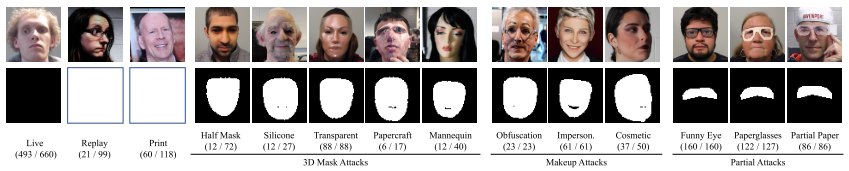
\includegraphics[width=1\textwidth]{img/report/Deep_tree_mask}
	\caption{حملات و ماسک‌های توجه\cite{Liu2019}}
	\label{fig:Deep_tree_mask}
	\centering
\end{figure}

برای اینکه بتواند دسته‌بندی مناسبی ارائه دهد نیاز به یک دادگان کامل است. به همین دلیل دادگان SiW-M که مدل توسعه داده شده از دادگان SiW است معرفی شد که شمال حملات بیشتری باشد. همچنین برای مقایسه نتیجه از دادگان‌های دیگری نیز استفاده شده‌ٰاست که در تصویر
\ref{fig:Deep_tree_dataset} 
مشاهده می‌کنید.
\begin{figure}[h]
	\centering
	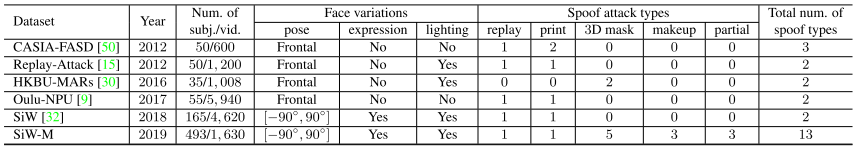
\includegraphics[width=1\textwidth]{img/report/Deep_tree_dataset}
	\caption{مقایسه دادگان مورد استفاده برای یادگیری مدل در برابر حملات جعل تصویر\cite{Liu2019}}
	\label{fig:Deep_tree_dataset}
	\centering
\end{figure} 

از ویژگی‌های این روش استفاده از داده زنده (تصویر واقعی) و تصویر جعل شده به طور همزمان در مدل در فرآیند یادگیری و تست است که کمتر در روش‌های قبلی مورد استفاده قرار می‌گرفته‌است. نتایج دقیق و تصویر‌سازی‌های حین و پس از فرآیند آموزش در مقاله قابل مشاهده‌است. نکته حائز اهمیت این مقاله استفاده از روش درختی‌ بر پایه یادگیری بدون نمونه و معرفی و استفاده از دادگان غنی است که کاربرد زیادی در کار ما می‌تواند داشته باشد.

\section{یادگیری بدون نمونه با مکانیزم توجه}
در مقاله (Dang2019) 
\cite{Dang2019} 
از ترکیب یادگیری بدون نمونه با استفاده از فرآیند توجه استفاده شده‌ که حائز اهمیت است. مکانیزم توجه به طور مثال در مدل‌های ترجمه متن ایجاد زیرنویس برای تصویر یا ویدیو کاربرد به سزایی دارد. انواع مکانیزم توجه وجود دارد به طور مثال در مقاله (Xu2015) 
\cite{Xu2015}
 از این مکانیزم برای تولید زیرنویس مناسب برای تصویر استفاده شده‌است. این مقاله بر روی حملات دستکاری دیجیتالی  تصویر تمرکز دارد و میٰخواهد تا با استفاده از یک نگاشت توجه مناسب همانند مقاله (Liu2019)
 \cite{Liu2019} 
 برای تشخیص ناحبه مورد جعل استفاده کند.
 
 همانطور که در تصویر 
 \ref{fig:Attention_face_anti_spoofing} 
 مشاهده می‌کنید مدل شبکه از دو بخش برای مقایسه تولید شده‌است. یک بخش که از یک یا چند لایه کانولوشن تشکیل شده و بخش دیگر که از ترکیب یک یا چند لایه کانولوشن به همراه لایه تمام متصل و دو نگاشت یکی نگاشت میانگین و دیگری مجموعه‌ای از نگاشت‌های پایه تشکیل شده است. در انتها خروجی هر کدام تحت عنوان نگاشت توجه به لایه sigmoid برای تصمیم‌گیری داده می‌شود.

برای  محاسبه نگاشت پایه یک عملیات PCA بر روی صد ماسک دستکاری شده از FaceApp انجام شده است و ده مولفه اول آن به عنوان نگاشت پایه و میانگین این مولفه‌ها به عنوان نگاشت میانگین در نظر گرفته می‌شود.
 \begin{figure}[h]
 	\centering
 	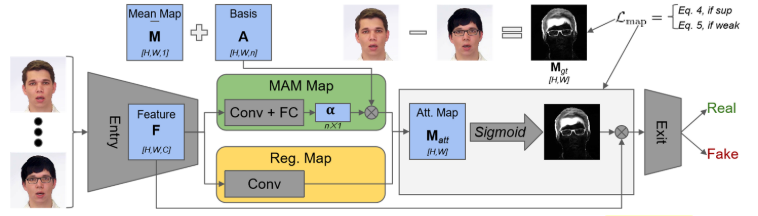
\includegraphics[width=1\textwidth]{img/report/Attention_face_anti_spoofing}
 	\caption{ساختار شبکه مورد استفاده برای یک سیستم تشخیص چهره\cite{Dang2019}}
 	\label{fig:Attention_face_anti_spoofing}
 	\centering
 \end{figure}
 
فرآیند یادگیری در سه حالت انجام شده‌است. در حالت اول برای هر حمله ماسک متناظر وجود دارد. (به طور کامل با نظارت) در حالت دوم برای برخی از داده‌ها ماسک متناظر وجود ندارد (نیمه نظارتی) و در حالت سوم هیچ ماسک متناظری وجود ندارد و فرآیند توجه باید خودش اطلاعات را به طور خودکار فرا بگیرد. (بدون ناظر)

برای اینکه یادگیری همه‌ جانبه باشد و انواع مختلفی از حملات را در بر گیرد یک دادگان از مجموع چند دادگان دیگر تولید شده‌است که مقایسه آن را در تصویر 
\ref{fig:Attention_face_anti_spoofing_dataset}
با دیگر دادگان استفاده شده در مقاله می‌توانید مشاهده کنید. 
 \begin{figure}[h]
	\centering
	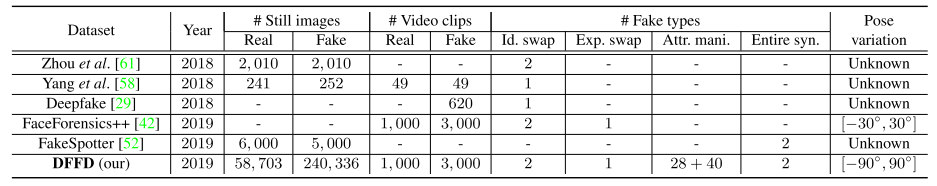
\includegraphics[width=1\textwidth]{img/report/Attention_face_anti_spoofing_dataset}
	\caption{ساختار شبکه مورد استفاده برای یک سیستم تشخیص چهره\cite{Dang2019}}
	\label{fig:Attention_face_anti_spoofing_dataset}
	\centering
\end{figure}

نکته حائز اهمیت در این مقاله استفاده از مکانیزم توجه به همراه یادگیری بدون نمونه بود که برای کار‌های زیادی به جز جلوگیری از جعل تصویر چهره می‌توان استفاده کرد. 

\section{جمع‌بندی}\label{sec:3جمع‌بندی}
در این بخش به معرفی چند کار مرتبط پرداختیم. روش‌های استفاده شده در این مقالات مانند: مکانیزم توجه به همراه یادگیری بدون نمونه، استفاده از درخت تصمیم و استفاده از شبکه‌های GAN برای تولید داده و دادگان معرفی شده توسط هر کدام را به طور مختصر مورد بررسی قرار دادیم. در ادامه و در فصل آینده درباره روش پیشنهادی و نقاط صعف و قوت این روش و روش‌های پیشین بحث خواهیم کرد.














